\documentclass[letterpaper,10pt, openright]{report}
\usepackage{lmodern}
\usepackage{amssymb,amsmath}
\usepackage{ifxetex,ifluatex}
\usepackage{fixltx2e} % provides \textsubscript
\ifnum 0\ifxetex 1\fi\ifluatex 1\fi=0 % if pdftex
  \usepackage[T1]{fontenc}
  \usepackage[utf8]{inputenc}
\else % if luatex or xelatex
  \ifxetex
    \usepackage{mathspec}
    \usepackage{xltxtra,xunicode}
  \else
    \usepackage{fontspec}
  \fi
  \defaultfontfeatures{Mapping=tex-text,Scale=MatchLowercase}
  \newcommand{\euro}{€}
\fi
% use upquote if available, for straight quotes in verbatim environments
\IfFileExists{upquote.sty}{\usepackage{upquote}}{}
% use microtype if available
\IfFileExists{microtype.sty}{%
\usepackage{microtype}
\UseMicrotypeSet[protrusion]{basicmath} % disable protrusion for tt fonts
}{}

% margenes segun reglas uchile
\headheight 36pt
\usepackage{geometry}
\geometry{verbose,letterpaper,tmargin=20mm,bmargin=20mm,lmargin=20mm,rmargin=35mm}
\parindent 0em
\parskip 2ex

\usepackage{color}
\usepackage{fancyvrb}
\newcommand{\VerbBar}{|}
\newcommand{\VERB}{\Verb[commandchars=\\\{\}]}
\DefineVerbatimEnvironment{Highlighting}{Verbatim}{commandchars=\\\{\}}
% Add ',fontsize=\small' for more characters per line
\usepackage{framed}
\definecolor{shadecolor}{RGB}{248,248,248}
\newenvironment{Shaded}{\begin{snugshade}}{\end{snugshade}}
\newcommand{\AlertTok}[1]{\textcolor[rgb]{0.94,0.16,0.16}{#1}}
\newcommand{\AnnotationTok}[1]{\textcolor[rgb]{0.56,0.35,0.01}{\textbf{\textit{#1}}}}
\newcommand{\AttributeTok}[1]{\textcolor[rgb]{0.77,0.63,0.00}{#1}}
\newcommand{\BaseNTok}[1]{\textcolor[rgb]{0.00,0.00,0.81}{#1}}
\newcommand{\BuiltInTok}[1]{#1}
\newcommand{\CharTok}[1]{\textcolor[rgb]{0.31,0.60,0.02}{#1}}
\newcommand{\CommentTok}[1]{\textcolor[rgb]{0.56,0.35,0.01}{\textit{#1}}}
\newcommand{\CommentVarTok}[1]{\textcolor[rgb]{0.56,0.35,0.01}{\textbf{\textit{#1}}}}
\newcommand{\ConstantTok}[1]{\textcolor[rgb]{0.00,0.00,0.00}{#1}}
\newcommand{\ControlFlowTok}[1]{\textcolor[rgb]{0.13,0.29,0.53}{\textbf{#1}}}
\newcommand{\DataTypeTok}[1]{\textcolor[rgb]{0.13,0.29,0.53}{#1}}
\newcommand{\DecValTok}[1]{\textcolor[rgb]{0.00,0.00,0.81}{#1}}
\newcommand{\DocumentationTok}[1]{\textcolor[rgb]{0.56,0.35,0.01}{\textbf{\textit{#1}}}}
\newcommand{\ErrorTok}[1]{\textcolor[rgb]{0.64,0.00,0.00}{\textbf{#1}}}
\newcommand{\ExtensionTok}[1]{#1}
\newcommand{\FloatTok}[1]{\textcolor[rgb]{0.00,0.00,0.81}{#1}}
\newcommand{\FunctionTok}[1]{\textcolor[rgb]{0.00,0.00,0.00}{#1}}
\newcommand{\ImportTok}[1]{#1}
\newcommand{\InformationTok}[1]{\textcolor[rgb]{0.56,0.35,0.01}{\textbf{\textit{#1}}}}
\newcommand{\KeywordTok}[1]{\textcolor[rgb]{0.13,0.29,0.53}{\textbf{#1}}}
\newcommand{\NormalTok}[1]{#1}
\newcommand{\OperatorTok}[1]{\textcolor[rgb]{0.81,0.36,0.00}{\textbf{#1}}}
\newcommand{\OtherTok}[1]{\textcolor[rgb]{0.56,0.35,0.01}{#1}}
\newcommand{\PreprocessorTok}[1]{\textcolor[rgb]{0.56,0.35,0.01}{\textit{#1}}}
\newcommand{\RegionMarkerTok}[1]{#1}
\newcommand{\SpecialCharTok}[1]{\textcolor[rgb]{0.00,0.00,0.00}{#1}}
\newcommand{\SpecialStringTok}[1]{\textcolor[rgb]{0.31,0.60,0.02}{#1}}
\newcommand{\StringTok}[1]{\textcolor[rgb]{0.31,0.60,0.02}{#1}}
\newcommand{\VariableTok}[1]{\textcolor[rgb]{0.00,0.00,0.00}{#1}}
\newcommand{\VerbatimStringTok}[1]{\textcolor[rgb]{0.31,0.60,0.02}{#1}}
\newcommand{\WarningTok}[1]{\textcolor[rgb]{0.56,0.35,0.01}{\textbf{\textit{#1}}}}
\usepackage{graphicx}
\makeatletter
\def\maxwidth{\ifdim\Gin@nat@width>\linewidth\linewidth\else\Gin@nat@width\fi}
\def\maxheight{\ifdim\Gin@nat@height>\textheight\textheight\else\Gin@nat@height\fi}
\makeatother
% Scale images if necessary, so that they will not overflow the page
% margins by default, and it is still possible to overwrite the defaults
% using explicit options in \includegraphics[width, height, ...]{}
\setkeys{Gin}{width=\maxwidth,height=\maxheight,keepaspectratio}
\ifxetex
  \usepackage[setpagesize=false, % page size defined by xetex
              unicode=false, % unicode breaks when used with xetex
              xetex]{hyperref}
\else
  \usepackage[unicode=true]{hyperref}
\fi
\hypersetup{breaklinks=true,
            bookmarks=true,
            pdfauthor={},
            pdftitle={},
            colorlinks=true,
            citecolor=blue,
            urlcolor=blue,
            linkcolor=magenta,
            pdfborder={0 0 0}}
\urlstyle{same}  % don't use monospace font for urls
\setlength{\parindent}{0pt}
\setlength{\parskip}{6pt plus 2pt minus 1pt}
\setlength{\emergencystretch}{3em}  % prevent overfull lines
\setcounter{secnumdepth}{0}

%%% Use protect on footnotes to avoid problems with footnotes in titles
\let\rmarkdownfootnote\footnote%
\def\footnote{\protect\rmarkdownfootnote}


  \title{}
    \author{}
    \date{}
  

% portada segun reglas uchile
\usepackage{multirow}

\renewcommand{\maketitle}{%
    \thispagestyle{empty}
    \renewcommand{\baselinestretch}{1}
    \begin{center}
    \begin{tabular}{ll}
        \multirow{3}{*}{\includegraphics[height=50pt]{figuras/escudo.pdf}}
        &\\
        &\large{\MakeUppercase{Universidad de Chile}}\\
        &\large{\MakeUppercase{LA FACULTAD}}\\
        &\large{\MakeUppercase{EL DEPARTAMENTO}}\\
        &\\
    \end{tabular}
    \end{center}
    \begin{center}
        %\vskip 2.75cm%
        \vfill
                        {\Large \bfseries \MakeUppercase{TESIS CON R RMARKDOWN, FALTAN INDICES Y TRUCOS CON BABEL}}\\
                                    {\Large  \bfseries \MakeUppercase{SUBTITULO DE LA TESIS}}\\
                    \vskip 0.75cm%
            {\large \MakeUppercase{TESIS PARA OPTAR AL GRADO DE}}\\
        \vfill
            {\large \MakeUppercase{AUTOR UNO}}\\
        \vskip 0.75cm%
            \large\MakeUppercase{Profesor Gu\'ia:}\\
            \large\MakeUppercase{PROFESOR GUIA}\\
        \vskip 0.75cm
                        \large\MakeUppercase{Comisi\'on Evaluadora:}\\
            \large\MakeUppercase{PROFESOR COMISION UNO}\\
                        \ifx PROFESOR COMISION DOS \undefined
                \vskip 0.33cm
                \vskip 11pt
            \else
                \large\MakeUppercase{PROFESOR COMISION DOS}\\
            \fi
            \ifx PROFESOR COMISION TRES \undefined
                \vskip 0.33cm
                \vskip 11pt
            \else
                \large\MakeUppercase{PROFESOR COMISION TRES}\\
            \fi
        \vfill
                \large\MakeUppercase{CIUDAD, PAIS}\\
                \large\MakeUppercase{MES ANIO}\\
        \vskip 1cm%
            \ifx FONDECYT NUMERO 123 \undefined
                {}
            \else
                \begin{footnotesize}
                    \begin{tabular}{c}
                        \hline
                        \\
                        FONDECYT NUMERO 123\\
                        \\
                        \hline
                    \end{tabular}
                \end{footnotesize}
            \fi
    \end{center}
    \newpage
}

\begin{document}

\maketitle


\hypertarget{nombre-del-capitulo-1}{%
\chapter{NOMBRE DEL CAPITULO 1}\label{nombre-del-capitulo-1}}

\hypertarget{seccion-1}{%
\section{SECCION 1}\label{seccion-1}}

Por completitud incluyo una cita en Bibtex: @bock2010stats.

Texto de ejemplo: Sed ut perspiciatis unde omnis iste natus error sit
voluptatem accusantium doloremque laudantium, totam rem aperiam, eaque
ipsa quae ab illo inventore veritatis et quasi architecto beatae vitae
dicta sunt explicabo. Nemo enim ipsam voluptatem quia voluptas sit
aspernatur aut odit aut fugit, sed quia consequuntur magni dolores eos
qui ratione voluptatem sequi nesciunt. Neque porro quisquam est, qui
dolorem ipsum quia dolor sit amet, consectetur, adipisci velit, sed quia
non numquam eius modi tempora incidunt ut labore et dolore magnam
aliquam quaerat voluptatem. Ut enim ad minima veniam, quis nostrum
exercitationem ullam corporis suscipit laboriosam, nisi ut aliquid ex ea
commodi consequatur? Quis autem vel eum iure reprehenderit qui in ea
voluptate velit esse quam nihil molestiae consequatur, vel illum qui
dolorem eum fugiat quo voluptas nulla pariatur?

\hypertarget{sub-seccion-1}{%
\section{SUB-SECCION 1}\label{sub-seccion-1}}

Texto de ejemplo: At vero eos et accusamus et iusto odio dignissimos
ducimus qui blanditiis praesentium voluptatum deleniti atque corrupti
quos dolores et quas molestias excepturi sint occaecati cupiditate non
provident, similique sunt in culpa qui officia deserunt mollitia animi,
id est laborum et dolorum fuga. Et harum quidem rerum facilis est et
expedita distinctio. Nam libero tempore, cum soluta nobis est eligendi
optio cumque nihil impedit quo minus id quod maxime placeat facere
possimus, omnis voluptas assumenda est, omnis dolor repellendus.
Temporibus autem quibusdam et aut officiis debitis aut rerum
necessitatibus saepe eveniet ut et voluptates repudiandae sint et
molestiae non recusandae. Itaque earum rerum hic tenetur a sapiente
delectus, ut aut reiciendis voluptatibus maiores alias consequatur aut
perferendis doloribus asperiores repellat.

\hypertarget{nombre-del-capitulo-2}{%
\chapter{NOMBRE DEL CAPITULO 2}\label{nombre-del-capitulo-2}}

\hypertarget{seccion-1-algunas-ecuaciones}{%
\section{SECCION 1: ALGUNAS
ECUACIONES}\label{seccion-1-algunas-ecuaciones}}

\hypertarget{serie-geometrica}{%
\subsection{Serie geométrica}\label{serie-geometrica}}

Sea \(r\in (0,1)\) se tiene que la suma de exponentes consecutivos de
\(r^i\) converge, es decir \begin{equation}
\sum_{i=0}^{\infty} r^i = \frac{1}{1-r}
\end{equation} notamos que \(r\) puede crecer de manera tal que \[
\lim_{r\to \infty} \frac{1}{1-r} = 0
\] o escrito de otra manera \[
\sum_{i=0}^{\infty} r^i = \frac{1}{1-r} \stackrel{r\to \infty}{\longrightarrow} 0
\]

\hypertarget{distribucion-normal}{%
\subsection{Distribución Normal}\label{distribucion-normal}}

\begin{equation}
\mathcal{N}(\mu,\sigma^2) = \int\limits_{-\infty}^{x} \frac1{\sigma\sqrt{2\pi}}\: \exp{-\frac{1}{2}\left(\frac{t-\mu}{\sigma}\right)^2}\: dt
\end{equation}

\appendix

\hypertarget{insertando-imagenes-tablas-codigo-etc}{%
\chapter{INSERTANDO IMAGENES, TABLAS, CODIGO,
ETC}\label{insertando-imagenes-tablas-codigo-etc}}

\hypertarget{r-markdown}{%
\section{R Markdown}\label{r-markdown}}

This is an R Markdown document. Markdown is a simple formatting syntax
for authoring HTML, PDF, and MS Word documents. For more details on
using R Markdown see \url{http://rmarkdown.rstudio.com}.

When you click the \textbf{Knit} button a document will be generated
that includes both content as well as the output of any embedded R code
chunks within the document. You can embed an R code chunk like this:

\begin{Shaded}
\begin{Highlighting}[]
\KeywordTok{summary}\NormalTok{(cars)}
\end{Highlighting}
\end{Shaded}

\begin{verbatim}
##      speed           dist       
##  Min.   : 4.0   Min.   :  2.00  
##  1st Qu.:12.0   1st Qu.: 26.00  
##  Median :15.0   Median : 36.00  
##  Mean   :15.4   Mean   : 42.98  
##  3rd Qu.:19.0   3rd Qu.: 56.00  
##  Max.   :25.0   Max.   :120.00
\end{verbatim}

\hypertarget{including-plots}{%
\section{Including Plots}\label{including-plots}}

You can also embed plots, for example:

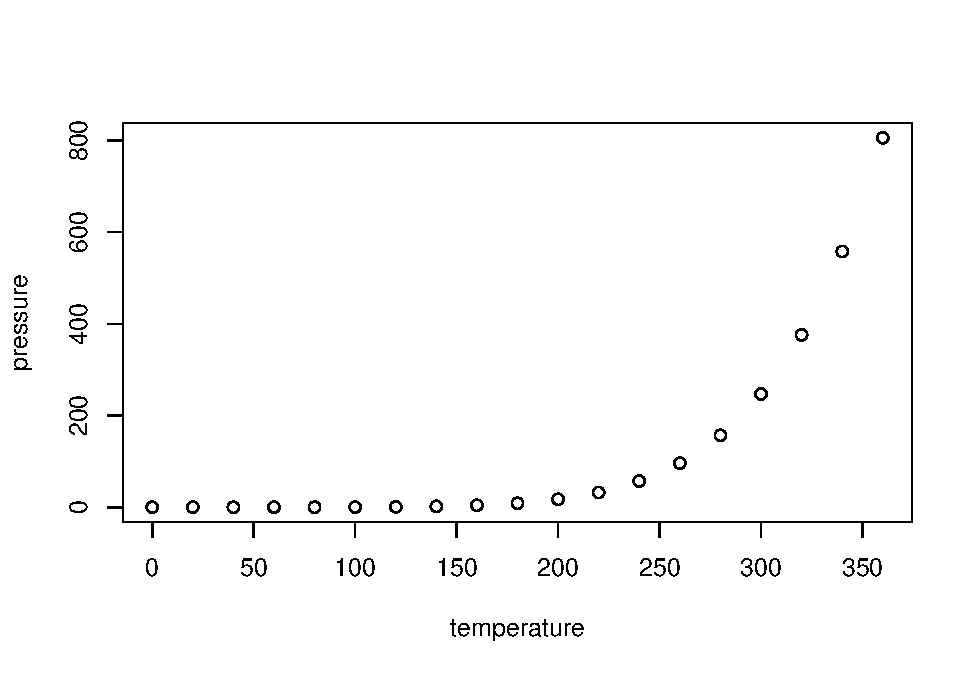
\includegraphics{rmarkdown-demo_files/figure-latex/pressure-1.pdf}

Note that the \texttt{echo\ =\ FALSE} parameter was added to the code
chunk to prevent printing of the R code that generated the plot.

\end{document}
